% !TeX root=../main.tex
\chapter{جزئیات فنی کالیبراسیون، شبیه‌سازی و سیم‌پیچ‌ها}
\label{app:technical-details}

این پیوست، ضرایب کالیبراسیون، تنظیمات اجرایی بینایی و شبیه‌ساز و پارامترهای سیم‌پیچ‌های نمونه را ثبت می‌کند. روش تخمین وضعیت در بخش~\ref{sec:method-vision} و معماری شبیه‌ساز در بخش~\ref{sec:method-sim-env} تشریح شده‌اند. مقادیر این پیوست، مشخصات نسخه‌ی مورد استفاده‌اند و به‌تنهایی ارزیابی دقت حسگر یا اعتبار فیزیکی مدل را تشکیل نمی‌دهند.

\section{کالیبراسیون درونی دوربین}
\label{sec:appendix-camera-calibration}

کالیبراسیون درونی با صفحه‌ی \lr{ChArUco} شامل $9\times6$ مربع، طول مربع $0.029\,\mathrm m$ و فرهنگ \lr{DICT\_6X6\_250} انجام شد. مجموعه‌ی ذخیره‌شده شامل 100 تصویر پذیرفته‌شده از 8235 فریم پردازش‌شده است و طول نشانگر کالیبراسیون $0.019\,\mathrm m$ در نظر گرفته شد. ماتریس درونی حاصل در معادله‌ی \ref{eq:method-camera-matrix} آمده است.

\begin{equation}
	K=\begin{bmatrix}
	601.6582&0&322.5702\\
	0&601.9886&240.8312\\
	0&0&1
	\end{bmatrix},
	\label{eq:method-camera-matrix}
\end{equation}

بردار اعوجاج در قرارداد شعاعی--مماسی \lr{OpenCV} نیز در معادله‌ی \ref{eq:method-camera-distortion} ارائه شده است.

\begin{equation}
	\mathbf d=[0.096912,-0.138412,0.004150,-0.003813,-0.346710]
	\label{eq:method-camera-distortion}
\end{equation}


\section{تنظیمات تصویربرداری و تخمین وضعیت}
\label{sec:appendix-vision-settings}

\begin{table}[!htbp]
	\centering
	\small
	\caption{تنظیمات دریافت و نمایش تصویر در نسخه‌ی مورد استفاده}
	\label{tab:appendix-camera-settings}
	\begin{tabular}{|p{0.45\textwidth}|p{0.38\textwidth}|}
		\hline
		پارامتر & مقدار\\ \hline
		رابط دوربین & \lr{Picamera2}\\ \hline
		وضوح تصویر & $640\times480$ پیکسل\\ \hline
		قالب تصویر & \lr{BGR888}\\ \hline
		نرخ اسمی & $30$ فریم‌برثانیه\\ \hline
		زمان نوردهی & $40000\,\mu\mathrm s$\\ \hline
		بهره‌ی آنالوگ & $10$\\ \hline
		خانواده‌ی نشانگر & \lr{tag36h1.81}\\ \hline
		طول ضلع سیاه نشانگر & $0.05\,\mathrm m$\\ \hline
		دوران تصویر نمایشی & $180^\circ$ پس از محاسبه‌ی هندسی\\ \hline
	\end{tabular}
\end{table}

دوران تصویر نمایشی در جدول~\ref{tab:appendix-camera-settings} تنها برای نمایش اعمال می‌شود و دستگاه مختصات تخمین وضعیت را تغییر نمی‌دهد.

حل اصلی با \lr{solvePnPRansac} و روش \lr{IPPE}، سقف 200 تکرار، آستانه‌ی بازفرافکنی 5 پیکسل و سطح اطمینان $0.999$ انجام می‌شود. در صورت ناموفق‌بودن حل مقاوم، حل \lr{IPPE} بدون \lr{RANSAC} آزموده می‌شود. انتقالی که بیش از $0.15\,\mathrm m$ با آخرین انتقال پذیرفته‌شده اختلاف داشته باشد رد می‌گردد.

ثبت دستگاه جهان به حضور هر چهار نشانگر ثابت در 15 فریم متوالی با حل موفق وابسته است؛ این شرط میانگین‌گیری تبدیل‌ها نیست. در ردیابی متحرک، حداقل سه نشانگر برای تصحیح اندازه‌گیری لازم است. پس از 30 فریم نامعتبر، حالت \lr{LOST} فعال می‌شود و انتشار وضعیت جدید متوقف می‌گردد. بازگشت مشاهده‌ی معتبر حداقل سه نشانگر، بازنشانی فیلتر و ازسرگیری انتشار را فعال می‌کند.

پارامترهای نویز فرایند برای موقعیت و سرعت در فیلتر کالمن به‌ترتیب $0.001$ و $0.01$ و پارامتر پایه‌ی نویز اندازه‌گیری $0.0001$ هستند. این اعداد، تنظیمات فیلتر پیاده‌سازی‌شده‌اند و به‌عنوان خطای اندازه‌گیری مستقل گزارش نمی‌شوند. عدم‌قطعیت اندازه‌گیری در مشاهده‌ی سه نشانگر نسبت به چهار نشانگر افزایش می‌یابد و سرعت بازنمایی‌شده به $2\,\mathrm{m/s}$ محدود است. هموارسازی زاویه‌ای از رابطه‌ی زیر پیروی می‌کند:

\begin{equation}
	\mathbf r_k=0.6\mathbf r_{k-1}+0.4\mathbf r_{m,k}
	\label{eq:method-orientation-filter}
\end{equation}


مقادیر پیش‌فرض ذخیره‌شده برای تصحیح ارتفاع، سمت‌گشت و تاب به‌ترتیب $+0.020\,\mathrm m$، $-0.57\,\mathrm{rad}$ و $+0.78\,\mathrm{rad}$ هستند. تصحیح‌های موقعیت و این دو زاویه از رابط کاربر قابل تنظیم‌اند و وضعیت جاری می‌تواند به‌عنوان مبدأ ثبت شود. برای غلت تصحیح مستقلی تعریف نشده است. مقادیر ذخیره‌شده، تنظیم هم‌راستایی نسخه‌ی مورد استفاده را ثبت می‌کنند و جایگزین سنجش مستقل دقت وضعیت نیستند.

\section{گره‌ها و رابط‌های اجرایی شبیه‌ساز}
\label{sec:appendix-ros-interfaces}

شکل~\ref{fig:results-ros2-graph} گراف محاسباتی \lr{ROS~2} را در حین اجرای شبیه‌سازی نشان می‌دهد که شامل گره‌ها و تاپیک‌های فعال است.

\begin{figure}[htbp]
	\centering
	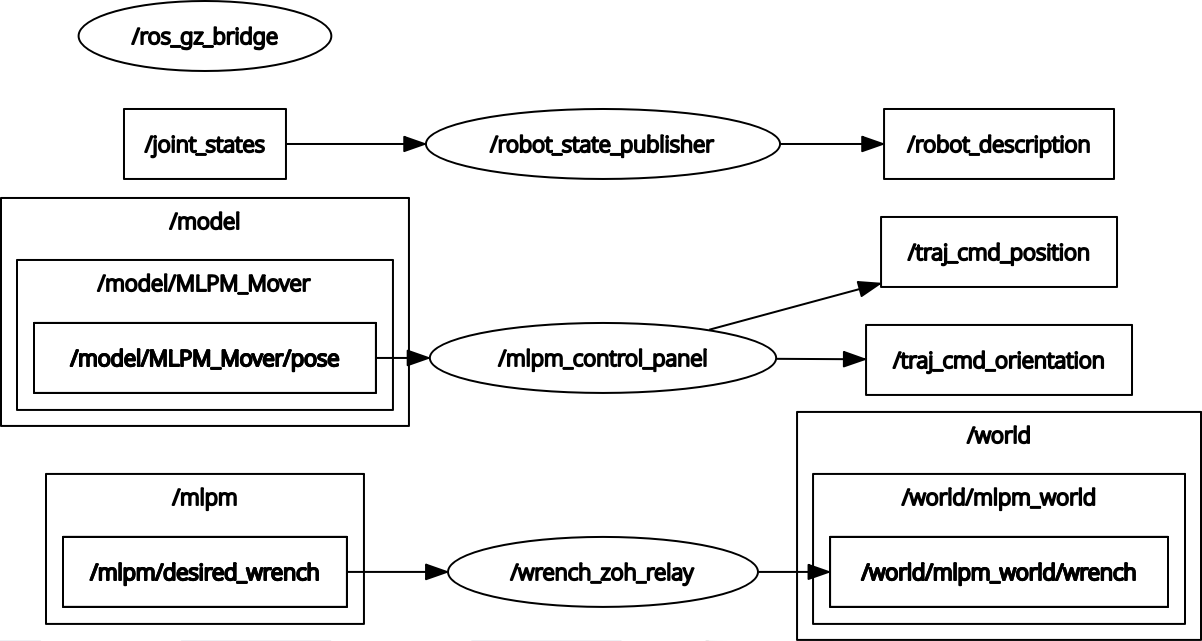
\includegraphics[width=0.95\textwidth]{img/ROS2_Topics.png}
	\caption{گراف محاسباتی \lr{ROS~2} در حین اجرای شبیه‌سازی \lr{MLPM}}
	\label{fig:results-ros2-graph}
\end{figure}

گره‌های اصلی نمایش‌داده‌شده در شکل~\ref{fig:results-ros2-graph} عبارت‌اند از:

\begin{itemize}
	\item \textbf{\lr{/mlpm\_control\_panel}}: گره رابط کنترل برای تولید و ارسال مرجع مسیر به \lr{MATLAB}؛
	\item \textbf{\lr{/wrench\_zoh\_relay}}: گره نگهدارنده‌ی مرتبه‌ی صفر برای حفظ فرمان پیچش میان نمونه‌های گسسته‌ی کنترل‌کننده؛
	\item \textbf{\lr{/ros\_gz\_bridge}}: چهار نمونه‌ی پل برای انتقال ساعت، وضعیت، پیچش و پارامترها میان \lr{Gazebo} و \lr{ROS~2}؛
	\item \textbf{\lr{/robot\_state\_publisher}}: انتشار توصیف هندسی ربات از \lr{URDF}.
\end{itemize}

تاپیک‌های کلیدی که در معماری ارتباطی نقش دارند در جدول~\ref{tab:results-ros-topics} خلاصه شده‌اند.

\begin{table}[htbp]
	\centering
	\caption{تاپیک‌های اصلی \lr{ROS~2} در محیط شبیه‌سازی}
	\label{tab:results-ros-topics}
	\scriptsize
	\begin{tabularx}{\textwidth}{@{}p{0.40\textwidth}p{0.30\textwidth}X@{}}
		\hline
		\textbf{تاپیک} & \textbf{نوع پیام} & \textbf{نقش} \\
		\hline
		\lr{/model/MLPM\_Mover/pose} & \lr{geometry\_msgs/Pose} & بازخورد وضعیت از \lr{Gazebo} \\
		\lr{/world/mlpm\_world/wrench} & \lr{geometry\_msgs/Wrench} & اعمال نیرو/گشتاور به پلتفرم \\
		\lr{/mlpm/desired\_wrench} & \lr{geometry\_msgs/Wrench} & پیچش مطلوب پیش از نگهدارنده‌ی مرتبه‌ی صفر \\
		\lr{/traj\_cmd\_position} & \lr{geometry\_msgs/Point} & مرجع موقعیت خطی \\
		\lr{/traj\_cmd\_orientation} & \lr{geometry\_msgs/Quaternion} & مرجع جهت‌گیری \\
		\hline
	\end{tabularx}
\end{table}


\section{تنظیمات اجرایی مدل در \lr{Gazebo}}
\label{sec:appendix-simulator-settings}

بستر مرحله‌ی مرجع با \lr{Gazebo Harmonic}، \lr{ROS~2 Jazzy} و موتور فیزیک \lr{DART} اجرا شد. مدل متحرک در قالب \lr{URDF/Xacro} تعریف شد و هندسه‌ی نمایشی از شبکه‌ی \lr{STL} آرایه‌ی هالباخ با ضریب مقیاس $0.001$ استفاده می‌کند. هندسه‌ی برخورد یک مکعب‌مستطیل با ابعاد $0.2286\times0.2286\times0.013\,\mathrm m$ است. پارامترهای دینامیکی مرجع در جدول~\ref{tab:method-reference-dynamics} گزارش شده‌اند.

\begin{table}[!htbp]
	\centering
	\caption{تنظیمات فیزیک و زمان‌بندی شبیه‌ساز مرجع}
	\label{tab:appendix-simulator-settings}
	\begin{tabular}{|p{0.45\textwidth}|p{0.38\textwidth}|}
		\hline
		پارامتر & مقدار\\ \hline
		گام فیزیک & $0.005\,\mathrm s$\\ \hline
		بردار گرانش در محیط & $[0,0,-9.8]^T\,\mathrm{m/s^2}$\\ \hline
		ضریب اصطکاک سطح تماس & $0.8$\\ \hline
		حد سرعت خطی & $10\,\mathrm{m/s}$\\ \hline
		حد سرعت زاویه‌ای & $5\,\mathrm{rad/s}$\\ \hline
		نرخ اسمی انتشار وضعیت & $60\,\mathrm{Hz}$\\ \hline
		دوره‌ی کنترل سیمولینک & $0.01\,\mathrm s$\\ \hline
	\end{tabular}
\end{table}

این حدود، تنظیمات محیط شبیه‌سازی‌اند و مشخصات اندازه‌گیری‌شده‌ی نمونه‌ی ساخته‌شده نیستند. نگهداری فرمان میان نمونه‌ها با گره‌های واسط انجام می‌شود تا تفاوت نرخ فیزیک، انتشار وضعیت و کنترل موجب قطع اعمال فرمان نشود.

\section{معیارهای اعتبارسنجی محیط شبیه‌سازی}
\label{sec:appendix-simulation-validation}

برای بررسی بستر شبیه‌سازی، موارد زیر کنترل شدند:
\begin{enumerate}
	\item \textbf{بارگذاری مدل}: مدل \lr{URDF} با پارامترهای جرمی و اینرسی تعریف‌شده در \lr{Gazebo} بارگذاری شد و در ارتفاع اولیه $z=4.0\,\mathrm m$ قرار گرفت.
	\item \textbf{همگام‌سازی زمان}: گره‌های \lr{ROS~2} زمان شبیه‌ساز را از تاپیک \lr{\texttt{/clock}} دریافت کردند.
	\item \textbf{بازخورد وضعیت}: وضعیت منتشرشده توسط \lr{\texttt{PosePublisher}} از طریق \lr{\texttt{parameter\_bridge}} به \lr{MATLAB} منتقل شد.
	\item \textbf{اعمال پیچش}: فرمان \lr{wrench} ارسالی از \lr{MATLAB} از طریق تاپیک \lr{\texttt{/world/mlpm\_world/wrench}} و پلاگین \lr{\texttt{ApplyLinkWrench}} به \lr{\texttt{base\_link}} اعمال شد.
	\item \textbf{نگه‌داری فرمان}: گره \lr{\texttt{wrench\_zoh\_relay}} فرمان جدید را با شماره‌ی توالی \lr{seq} تشخیص داد و آن را میان نمونه‌های کنترل‌کننده ثابت نگه داشت.
	\item \textbf{پایداری عددی}: با تنظیمات جدول~\ref{tab:appendix-simulator-settings}، شبیه‌سازی در سناریوهای آزمایش بدون واگرایی عددی اجرا شد.
\end{enumerate}

\section{مختصات و مشخصه‌های سیم‌پیچ‌های فعال}
\label{sec:appendix-coil-parameters}

\begin{table}[!htbp]
	\centering
	\caption{مختصات مدل و ترتیب سخت‌افزاری سیم‌پیچ‌های فعال}
	\label{tab:method-active-coordinates}
	\begin{tabular}{|c|c|c|c|}
		\hline
		\textbf{ترتیب راه‌انداز} & \textbf{شماره‌ی سیم‌پیچ} & $x_c\,(\mathrm m)$ & $y_c\,(\mathrm m)$\\ \hline
		1&2&$-0.004$&$-0.112$\\ \hline
		2&6&$-0.024$&$-0.044$\\ \hline
		3&7&$+0.044$&$-0.024$\\ \hline
		4&8&$+0.112$&$-0.004$\\ \hline
		5&9&$-0.112$&$+0.004$\\ \hline
		6&10&$-0.044$&$+0.024$\\ \hline
		7&11&$+0.024$&$+0.044$\\ \hline
		8&15&$+0.004$&$+0.112$\\ \hline
	\end{tabular}
\end{table}

مدل هندسی هر سیم‌پیچ از ابعاد خارجی $68\times68\,\mathrm{mm}$، دهانه‌ی داخلی $20\times20\,\mathrm{mm}$، قطر هادی بدون عایق $0.8\,\mathrm{mm}$ و گام هادی عایق‌شده $0.85\,\mathrm{mm}$ استفاده می‌کند. مقاومت نامی در مدل $5.75\,\Omega$ و ضریب تراکم سیم‌پیچی $0.72$ است. برای لحاظ‌کردن ناهمسانی ساخت، مقاومت و اندوکتانس سیم‌پیچ‌ها اندازه‌گیری شد و طول هادی به‌جای فرض تعداد دور یکسان از مقاومت برآورد گردید:
\begin{equation}
	\ell_w=\frac{(R-R_{lead})A_w}{\rho},
	\qquad A_w=\pi\left(\frac{d_w}{2}\right)^2.
	\label{eq:method-wire-length}
\end{equation}

با تقریب $\ell_{turn}=x_{in}+x_{out}+y_{in}+y_{out}$، تعداد دور و ضخامت بسته‌ی سیم‌پیچ از رابطه‌های زیر به دست آمدند:
\begin{equation}
	N=\frac{\ell_w}{\ell_{turn}},
	\qquad
	t_w=\frac{\ell_wA_w}{k_pA_{plan}},
	\qquad
	A_{plan}=x_{out}y_{out}-x_{in}y_{in}
	\label{eq:method-winding-inference}
\end{equation}

برای سیم‌پیچ نامی $5.75\,\Omega$، طول هادی $102.492\,\mathrm m$، تعداد دور $582.339$ و ضخامت بسته $16.940\,\mathrm{mm}$ برآورد شد. این مقادیر اندازه‌گیری مستقیم نیستند و تنها برای مدل سیم‌پیچ محدود استفاده می‌شوند. مقاومت ویژه‌ی استفاده‌شده $2.82\times10^{-8}\,\Omega\,\mathrm m$ است.

\begin{table}[!htbp]
	\centering
	\scriptsize
	\caption{مشخصه‌های الکتریکی و پارامترهای تخمینی سیم‌پیچ‌های فعال}
	\label{tab:method-active-coil-properties}
	\begin{tabular}{|c|c|c|c|c|c|}
		\hline
		\textbf{سیم‌پیچ} & $L\,(\mathrm{mH})$ & $R_{0.1\mathrm{kHz}}\,(\Omega)$ & $N$ تخمینی & $t_w\,(\mathrm{mm})$ & $L/R\,(\mathrm{ms})$\\ \hline
		2&15.252&6.09&616.344&17.929&2.504\\ \hline
		6&14.113&5.84&591.962&17.219&2.417\\ \hline
		7&10.328&4.88&500.227&14.551&2.116\\ \hline
		8&17.517&6.58&663.190&19.291&2.662\\ \hline
		9&17.015&6.48&653.370&19.006&2.626\\ \hline
		10&11.058&5.09&519.844&15.122&2.173\\ \hline
		11&12.652&5.51&559.490&16.275&2.296\\ \hline
		15&13.966&5.8276&589.788&17.156&2.397\\ \hline
	\end{tabular}
\end{table}
